

\begin{frame}{Machine Learning Models}

    The algorithms we chose to train our models were:
    \begin{itemize}
        \item \textbf{Logistic Regression(LR):} Good with binary data, easy and simple to understand
        \item \textbf{Decision Tree(DT):} Decently robust to imbalanced datasets and irrelevant features
        \item \textbf{K Nearest Neighbours(KNN):} Overall simple
        \item \textbf{Random Forest(RF):} Handles imbalanced datasets well and is impervious to overfitting
        \item \textbf{Multilayer Perceptron(MLP):} Very powerful all arround
    \end{itemize}
    
    \textbf{Notes:}
    \begin{itemize}
        \item KNN was only tested with smaller data sets due to elevated training and testing times (lack of processing power)
        \item Logistic Regression was tested with a dataset where a column had been removed, in an attempt to fight the algorithm's sensitivity to irrelevant features
        \item All algorithms but MLP were tested with Grid Search with portions of the data set, in order to find the best parameters for the final model
    \end{itemize}
\end{frame}

\begin{frame}{Model Evaluation and Comparison}
    \begin{center}
        \scalebox{0.65}{
            \begin{table}[]
        \begin{tabular}{|l|l|l|l|l|l|l|l|}
        \hline
        \textbf{Model}             & \textbf{Time to train (s)} & \textbf{Time to test (s)} & \textbf{Recall}   & \textbf{Roc Auc}  & \textbf{Precision} & \textbf{Accuracy} & \textbf{Balanced Accuracy} \\ \hline
        lr\_control\_full & 19.497249         & 0.005409         & 0.599163 & 0.796077 & 0.890613  & 0.95874  & 0.796077          \\ \hline
        lr\_smoted\_full  & 55.498035          & 0.015769         & 0.980637 & 0.943067 & 0.497086  & 0.912032 & 0.943067          \\ \hline
        lr\_weight\_full  & 120.202866        & 0.016395         & 0.97291  & 0.94429  & 0.523563  & 0.920648 & 0.94429           \\ \hline
        dt\_control\_full & 12.073779         & 0.008223         & 0.999908 & 0.999952 & 0.999954  & 0.999988 & 0.999952          \\ \hline
        dt\_smoted\_full  & 26.15653          & 0.016174         & 0.999862 & 0.999922 & 0.999816  & 0.999972 & 0.999922          \\ \hline
        dt\_weight\_full  & 6.897408          & 0.015349         & 0.999908 & 0.999952 & 0.999954  & 0.999988 & 0.999952          \\ \hline
        mlp\_normal\_full & 960.845785        & 0.208947         & 0.892052 & 0.945036 & 0.977226  & 0.988804 & 0.945036          \\ \hline
        rf\_control\_full & 361.549095        & 1.325936         & 0.999908 & 0.999954 & 1         & 0.999992 & 0.999954          \\ \hline
        rf\_smoted\_full  & 132.806744        & 0.117373         & 0.999908 & 0.99995  & 0.999908  & 0.999984 & 0.99995           \\ \hline
        rf\_weight\_full  & 303.098518        & 0.771723         & 0.999908 & 0.999952 & 0.999954  & 0.999988 & 0.999952          \\ \hline
        knn\_control\_10p & 19.848561         & 47.906985        & 0.828354 & 0.904025 & 0.79605   & 0.966481 & 0.904025          \\ \hline
        knn\_smoted\_10p  & 233.760107        & 181.564677       & 0.989553 & 0.993826 & 0.980322  & 0.997353 & 0.993826          \\ \hline
        knn\_none\_10p    & 119.013859        & 121.487901       & 0.983827 & 0.991484 & 0.990951  & 0.997803 & 0.991484          \\ \hline
        \end{tabular}
        \end{table}
                }
    \end{center}
    
    \textbf{Note:} \textbf{control} are models trained with default parameters, \textbf{weight} are models trained on normal data sets but best parameters in grid search (focusing fixing the imbalance with class weights), \textbf{smote} are models trained with best parameters from grid search and using \textbf{SMOTE} in training data set, \textbf{none} is the same as weight but without class weights (for parameter details, check notebook)
\end{frame}

\begin{frame}{Model Evaluation and Comparison}


\begin{figure}
    \centering
    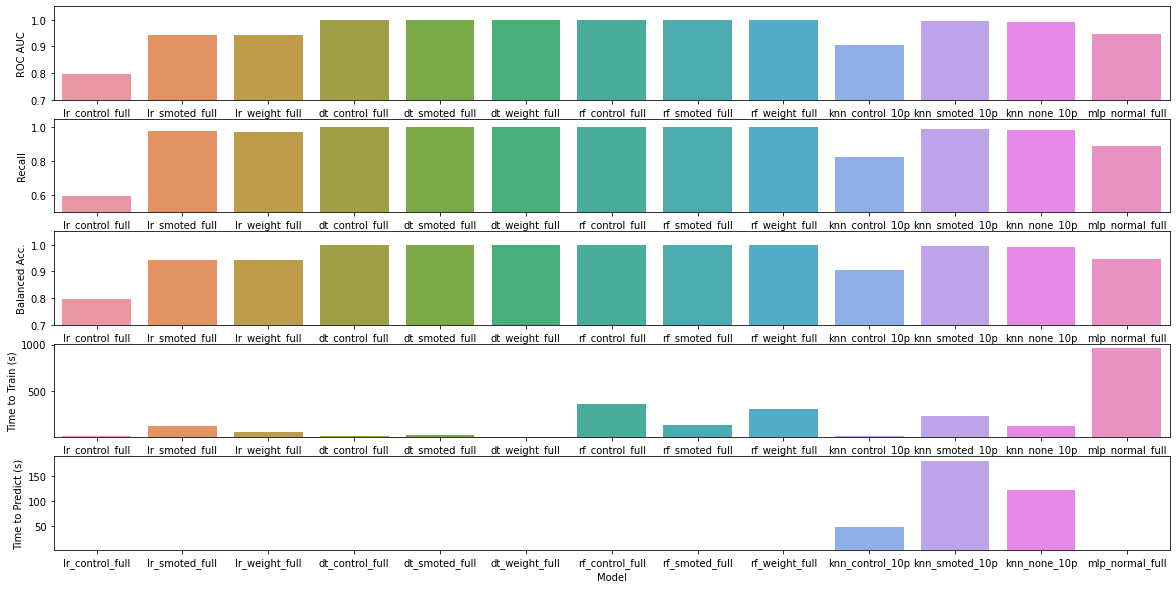
\includegraphics[width=.85\textwidth]{images/plots.png}
    \caption{Model Scores and Times}
    \label{fig:my_label}
\end{figure}
\end{frame}